\documentclass[border=8pt]{standalone}
\usepackage{fontspec}
\usepackage{unicode-math}
\usepackage{tikz}
\setmainfont{DejaVuSerif.ttf}
\setmathfont{latinmodern-math.otf}
\begin{document}
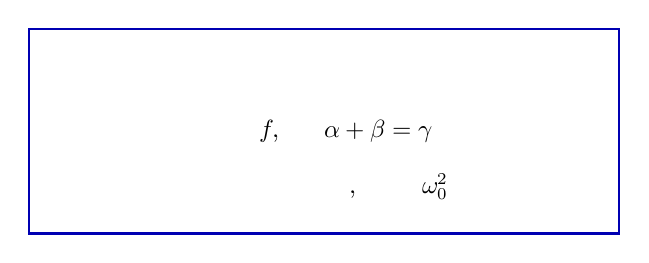
\begin{tikzpicture}[every node/.style={font=\small}]
  \draw[thick, blue!70!black] (0,0) rectangle (7.5,2.6);
  \node[font=\bfseries\small] at (3.75,2.0) {Оптика и квантовая яма};
  \node at (3.75,1.3) {Фокус $f$, угол $\alpha + \beta = \gamma$};
  \node at (3.75,0.6) {Греческие символы αβγ, частота $\omega_0^2$};
\end{tikzpicture}
\end{document}
